\chapter{Mean-Variance QTL Mapping Identifies Novel QTL for Circadian Activity and Exploratory Behavior in Mice}
\label{chap:mvqtl_reanalyses}

\section{Statistical Methods}

\subsection{Traditional QTL mapping based on the standard linear model (SLM)}

    The traditional approach to mapping a quantitative trait in an experimental cross with no population structure (\eg an F2 intercross or backcross) involves fitting, at each locus in turn, a linear model of the following form. Letting $y_i$ denote the phenotype value of individual $i$, this phenotype is modeled as
    \[
        y_i \sim \N(m_i,\, \sigma^2)\,,
    \]
    where $\sigma^2$ is the residual variance, and the expected phenotype mean, $m_i$, is predicted by effects of QTL genotype and, optionally, effects of covariates. In the reanalyses performed here, $m_i$ is modeled to include a covariate of sex and additive and dominance effects of QTL genotype, that is,
    \[
        m_i = \mu + \text{sex}_i\beta_\text{sex} + a_i\beta_a + d_i\beta_d\,,
    \]
    where $\mu$ is the intercept, $\beta_\text{sex}$ is the sex effect, with $\text{sex}_i$ indicating (0 or 1) the sex of individual $i$, and $\beta_a$ and $\beta_d$ are the additive and dominance effects of a QTL whose genotype is represented by $a_i$ and $d_i$ defined as follows: when QTL genotype is known, $a_i$ is the count (0,1,2) of one parental allele, and $d_i$ indicates heterozygosity (0 or 1); when QTL genotype is inferred based on flanking marker data, as is done here, $a_i$ and $d_i$ are replaced by their corresponding probabilistic expectations \citep{Haley1992,Martinez1992}. The evidence for association at a given putative QTL is based on a comparison of the fit of the model above with that of a null model that is identical except for the QTL effects being omitted. These models and their comparison we henceforth refer to as the standard linear model (SLM) approach.

\subsection{Mean-variance QTL mapping based on the double generalized linear model (DGLM)}

    The statistical model underlying mean-variance QTL mapping, the double generalized linear model (DGLM; \citealt{Smyth1989} and \citealt{Ronnegard2011a}), elaborates the SLM approach by modeling a potentially unique value of $\sigma^2$ for each individual, as
    \[
        y_i \sim \N(m_i, \,\sigma_i^2)\,,
    \]
    where $m_i$ has the same meaning as in the SLM, but now $\sigma^2_i$ is linked to its own linear predictor $v_i$ as
    \[
        \sigma_i = \exp(v_i),
    \]
    where the exponentiation ensures that $\sigma_i$ is always positive, though $v_i$ is unconstrained.
    The linear predictors for $m_i$ and $v_i$ are modeled as
    \begin{equation}\label{eq:dglm_full}
    \begin{aligned}
        \text{mean:~~~} m_i &= \mu + \text{sex}_i\beta_\text{sex} + a_i\beta_a + d_i\beta_d\\
        \text{log(variance):~~~} v_i &=  \mu_v + \text{sex}_i\gamma_\text{sex} + a_i\gamma_a + d_i\gamma_d
    \end{aligned}
    \end{equation}
    where $\mu$, $a_i$, $d_i$, $\text{sex}_i$, and the $\beta$'s are as before,
    $\mu_v$ is an intercept representing the (log of the) ``baseline'' residual variance, and $\gamma_a$, $\gamma_d$, and $\gamma_\text{sex}$ are the effects of the QTL and covariates on $v_i$.
    % As before, a representative example is described here, but other genetic parametrizations and additional covariates could be included straightforwardly.

    The evidence for a QTL association is now defined through three distinct model comparisons, corresponding to testing for an mQTL, a vQTL, or an mvQTL.
    In each case, the fit of the ``full'' model in \autoref{eq:dglm_full} is compared with that of a different fitted null: for the mQTL test, the null model omits the QTL effects on the mean (\ie, $\beta_a=\beta_d=0$); for the vQTL test, the null model omits the QTL effects on the variance (\ie, $\gamma_a=\gamma_d=0$); and for the mvQTL test, the null model omits QTL effects on both mean and variance (\ie, $\beta_a=\beta_d=\gamma_a=\gamma_d=0$).
    These tests are detailed in \CortyMethodsPaper.


\subsection{Genomewide significance and FWER-adjusted p-values}

The model comparisons described above constitute the SLM test and the three DGLM-based tests and each produces a likelihood ratio (LR) statistic.
These LR statistics are converted to $p$-values that are adjusted for the family-wise error rate (FWER) across loci, \ie, $p$-values on the scale of genomewide significance.
This adjustment is performed separately for each test by calculating an empirical distribution for the LR statistic under permutation, much in the spirit of \citet{Churchill1994} but with some modifications, namely that different tests have differently structured permutations.
Briefly, let $G_i$ be the full set of genetic information for individual $i$, that is, the genotypes or genotype probabilities across all loci.
For the SLM and mvQTL tests, we define a permutation as randomly shuffling the $G_i$'s across individuals; for the mQTL test, the permutations apply this shuffle only to the genotype information in the full model's mean component; for the vQTL test, the permutations apply the shuffle only to the genotype information in the full model's variance component.
For a given test, for each permutation we calculate LR statistics across the genome and record the maximum; the maxima of over all permutations is fitted to a generalized extreme value distribution, and the upper tail probabilities of this fitted distribution are used to calculated the FWER-adjusted $p$-values for the LR statistics in the unpermuted data [see \citealt{Dudbridge2004}, and, \eg, \citealt{Valdar06cc}; more details in \CortyMethodsPaper].
An FWER-adjusted $p$-value can be interpreted straightforwardly: it is the probability of observing an association statistic this large or larger in a genome scan of a phenotype with no true associations.

\subsection{Data Availability}

    All data and scripts used to conduct the analyses presented here and plot results are archived in a public, static repository at with DOI: \texttt{10.5281/zenodo.1187195}.
    Specifically, the raw data files are:

    \begin{itemize}
        \item \texttt{1\_Kumar2014.csv} The phenotype and genotype data from \citet{Kumar2013} that was reanalyzed.
            This dataset is also available from the Mouse Phenome Database \citep{Bogue2015} at \url{https://phenome.jax.org/projects/Kumar1}.
        \item \texttt{4\_Bailey2008.csv} The phenotype and genotype data from \citet{Bailey2008} that was reanalyzed.
            This dataset is also available from the Mouse Phenome Database at \url{https://phenome.jax.org/projects/Bailey1}.
        \item \texttt{9\_actogram\_data} The raw data on circadian activity from \citet{Kumar2013} that was used to plot actograms
    \end{itemize}
    The analysis and plotting scripts are:
    \begin{itemize}
        \item \texttt{2\_run\_Kumar\_scans.R} This script runs genome scans with \texttt{R/qtl} and \texttt{R/vqtl} on the data from \citet{Kumar2013}.
        \item \texttt{3\_plot\_Kumar\_scans.R} This script plots the results of the reanalysis of \citet{Kumar2013}.
        \item \texttt{5\_run\_Bailey\_scans.R} This script runs genome scans with \texttt{R/qtl} and \texttt{R/vqtl} on the data from \citet{Bailey2008}.
        \item \texttt{6\_plot\_Bailey\_scans.R} This script plots the results of the reanalysis of \citet{Bailey2008}.
        \item \texttt{7\_prune\_big\_files.R} This script strips out redundant information from the results to make the file size smaller to share more easily online.
        \item \texttt{8\_power\_simulations.R} This script runs the power simulation comparing the DGLM to the SLM at the QTL identified in the Kumar reanalysis.
    \end{itemize}

    The results of running the analysis and plotting scripts are:
    \begin{itemize}
        \item \texttt{Kumar\_scans\_1000\_perms.RDS} This file contains the results of the reanalysis of \citet{Kumar2013}.
        \item \texttt{Bailey\_scans\_1000\_perms.RDS} This file contains the results of the reanalysis of \citet{Bailey2008}.
        \item \texttt{Kumar\_plots} This directory contains the figures generated by \texttt{3\_plot\_Kumar\_scans.R} 
            (Figures \ref{fig:kumar_scan}, \ref{fig:kumar_detail}, and \ref{fig:replicate_kumar}).
        \item \texttt{Bailey\_plots} This directory contains the figures generated by \texttt{6\_plot\_Bailey\_scans.R}
            (Figures \ref{fig:bailey_scan_rearing}, \ref{fig:bailey_detail}, \ref{fig:Bailey_replicate}, \ref{fig:Bailey_rint_scans}, \ref{fig:Bailey_bc_scans}, and \ref{fig:Bailey_totrear_transforms}) 
    \end{itemize}



% \section{QTL Mapping Procedure}
%     We used the following procedure to reanalyze the datasets from \citealt{Leamy2000} and \citealt{Bailey2008}.
%     \begin{enumerate}
%         \item Fit the standard linear model to the phenotype with all suspected covariates, subject to standard limitations of linear regression.
%         Keep the ones that meet a modest threshold for statistical significance in step 1 (\eg $p < 0.1$ by the likelihood ratio test).
%         \item With the covariates from step 1, apply the Box-Cox procedure to find an appropriate transform for the phenotype \citep{Ronnegard2011a}.
%         \item Fit the DGLM to the transformed phenotype with all covariates from step 1 in both the mean and variance sub-model.
%         Within each sub-model, keep the covariates that meet a modest threshold for statistical significance.
%         \item Conduct a primary genome scan using the mean-variance QTL mapping approach to test for mQTL, vQTL, and mvQTL with the transformed phenotype from step 3 and the covariates from step 4.
%         \item Conduct 1000 permutation scans to evaluate the statistical significance of the observed associations.
%         To control experiment-wise error rate to approximately 0.05, aim for a family-wise error rate of 0.02 for each type of QTL (mQTL, vQTL, and mvQTL).
%         \item If any QTL were detected, add those QTL as covariates and scan again.
%         When an mQTL or mvQTL is detected, add the most associated genetic locus or pseudo-locus (not necessarily a marker) as a covariate in the mean sub-model.
%         When a vQTL or mvQTL is detected, add the most associated locus or pseudo-locus as a covariate in the variance sub-model.
%         \item Investigate QTL with the mean variance plot.
%     \end{enumerate}


\section{Reanalysis of Kumar et al. Reveals a new mQTL for Circadian Wheel Running Activity}
    % We used the double generalized linear model (DGLM) to reanalyze a reduced complexity cross between C57BL/6J and C57BL/6N mice in which cocaine response traits and circadian activity were measured.
    % The SLM identified one QTL on chromosome 11 for the cocaine response traits but no QTL related to the circadian activity were reported \citep{Kumar2013}.
    % The DGLM reanalysis identified the same QTL on chromosome 11 for the cocaine response traits and an additional QTL for a circadian activity trait on chromosome 6.

    \subsection{Summary of Original Study}

    \citet{Kumar2013} intercrossed C57BL/6J and C57BL/6N, two closely-related strains of C57BL6 that diverged in 1951, approximately 330 generations ago.
    Due to recent coancestry of the parental strains, this cross is termed a ``reduced complexity cross'', and their limited genetic differences ensure that any identified QTL region can be narrowed to a small set of variants bioinformatically.
    % The limited genetic variance allows the causative variants underlying any discovered QTL to be mapped with very high precision.
    % They termed such a cross a ``reduced complexity cross'' because, owing to their recent coancestry, the parental strains have very limited genetic differences, and thus any phenotype that is found to differ significantly between the strains can be mapped precisely and at low cost.
    The intercross resulted in 244 F2 offspring, 113 female and 131 male, which were tested for acute locomotor response to cocaine (20mg/kg) in the open field.
    One to three weeks following psychostimulant response testing, the mice were tested for circadian wheel running activity.

    Analysis of wheel running data was carried out using ClockLab software v6.0.36.
    % For , the ``scaled'' Y axis between 0 and 100 has been used.
    For calculation of activity 20 day epoch in DD was used in order to have standard display between actograms.
    % The activity data is presented in revolutions per minute (rev/min) during this 20 day epoch in DD.
    Analysis of other circadian measures such as period (tau) or amplitude were carried out using methods previously described \citep{Shimomura2001}.
    All animal protocols were approved by the Institutional Animal Care and Use Committee (IACUC) of the University of Texas Southwestern Medical Center

    Traditional QTL mapping with the SLM, reported in \citet{Kumar2013}, detected a single large-effect QTL for cocaine-response traits on chromosome 11, but no QTL for circadian activity.
    A later study by another group nonetheless observed that the circadian activity of the two strains showed significant differences \citep{Banks2015}.


    \subsection{Reanalysis with traditional QTL mapping and mean-variance QTL mapping}

    For the cocaine response traits, traditional QTL mapping and mean-variance QTL mapping
    gave results that were nearly identical to the originally-published analysis in \citet{Kumar2013} (\autoref{fig:replicate_kumar}). 

    For the circadian wheel running activity trait, however, traditional QTL mapping identified no QTL (\autoref{fig:kumar_scan} in green) but mean-variance QTL mapping identified one QTL on chromosome 6 (\autoref{fig:kumar_scan} in blue, black, and red).
    In this case, all three tests were statistically significant, but the most significant was the mQTL test (blue), so we discuss it as an mQTL.
    The most significant genetic marker was rs30314218 on chromosome 6, at 18.83 cM, 40.0 Mb, with a FWER-controlling $p$-value of 0.0063.
    The mQTL explains 8.4\% of total phenotype variance by the traditional definition of percent variance explained (\eg, \citealt{Broman2009}).

    \begin{figure*}
      \includegraphics[width=\linewidth]{images/Kumar_avg_counts_scan.pdf}
      \caption[
      Genome scan for Kumar et al. circadian wheel running activity.
      ]
      {
        Genome scan for Kumar et al. circadian wheel running activity.
        The horizontal axis shows chromosomal location and the vertical axis shows FWER-controlling $p$-values for the association between each genomic locus and circadian wheel running activity.
      }
      \label{fig:kumar_scan}
    \end{figure*}


    \subsection{Understanding the Novel QTL}
    Though they test for the same pattern, the mQTL test of mean-variance QTL mapping identified a QTL where the traditional QTL test did not.
    This discordance may arise when there is variance heterogeneity in the mapping population.
    In this case, mice homozygous for the C57BL/6N allele at the mQTL have both higher average wheel running activity and lower residual variance in wheel running activity than mice with other genotypes (\autoref{fig:kumar_phenotype_plot}).

    The identification of this QTL by mean-variance QTL mapping but not traditional QTL mapping can be understood by contrasting how the DGLM and SLM fit the data at this locus.

    For the SLM, a single value of the residual standard deviation $\sigma$ is estimated for all mice.
    Approximately 25\% of the mice are homozygous for the C57BL/6N allele, so $\sigma$ is estimated mostly based on heterozygous mice and homozygous C57BL/6J mice.
    The SLM estimates $\hat{\sigma}=7.83$, a slight underestimate for some genotype-sex combinations, and a drastic overestimate for the homozygous C57BL/6N of both sexes (\autoref{fig:kumar_meanvar_plot}).
    With $\sigma$ overestimated for the C57BL/6N homozygotes, the addition of a locus effect to the null model results in only a limited increase in the likelihood, one that could reasonably be caused by chance alone.
    For the DGLM, six different values of $\sigma$ are estimated, one for each genotype-sex combination (\autoref{fig:kumar_meanvar_plot}).
    With an better-estimated (lower) $\widehat{\sigma}$ for the C57BL/6N homozygotes, the addition of the locus effect to the null model results in a greater increase in the likelihood, one that is very unlikely due to chance alone.

    A simulation based on the estimated coefficients shows that at a false positive rate of $5 \times 10^{-4}$, relevant for genome-wide significance testing, the SLM has 61\% power to reject the null at this locus and the DGLM has 90\% power (See file \texttt{8\_power\_simulations.R}).

    \subsection{Variant Prioritization}
    Reduced complexity crosses allow variant prioritization to proceed quickly because of the number of segregating variants is small.
    Using 1000 nonparametric bootstrap resamples, the QTL interval was estimated as 13.5-23.5 cM (90\% CI), which translates to physical positions of 32.5 - 48.5 Mb using Mouse Map Converter's sex averaged Cox map \citep{Cox2009}.
    Since this interval contains no genes or previously identified QTL shown to regulate circadian rhythms, we prioritized candidates by identifying variants between C57BL/6J and C57BL/6NJ based on Sanger mouse genome database \citep{Keane2011a,Simon2013}, which yielded 463 SNPs, 124 indels, and 3 structural variants (\autoref{tab:kumar_variants}).
    % (cite https://genomebiology.biomedcentral.com/articles/10.1186/gb-2013-14-7-r82 and the variant query tool http://www.sanger.ac.uk/sanger/Mouse_SnpViewer/rel-1505). 
    
    Of these variants, none of the indels or structural variants were nonsynonymous.
    Two SNPs were predicted to lead to missense changes (T to A at position 6: 39400456 in \textit{Mkrn1}, and A to A/C at 6:48486716 in \textit{Sspo}).
    The variant in Sspo was a very low confidence call and therefore likely a false positive.

    The \textit{Mkrn1} (makorin ring finger protein 1) variant is a mutation in C57BL/6J that changes a highly conserved (\autoref{fig:mkrn1_alignment} and \autoref{fig:mkrn1_alignment2}) tyrosine to asparagine.
    It was determined to be the best candidate variant in the QTL interval.
    The Mkrn1 protein is a ubiquitin E3 ligase with zinc finger domains with poorly defined function \citep{Kim2005a}.
    It is expressed at low levels widely in the brain according to Allen Brain Atlas and EBI Expression Atlas \citep{Kapushesky2009,McWilliam2013,AllenInstituteforBrainScience2015,McWilliam2013}.
    Functional analysis will be necessary to experimentally confirm that this variant in Mkrn1 is indeed the causative mutation that led, in a dominant fashion, to the decreased expected value and increased variance of circadian wheel running activity observed in mice with at least one copy of the C57BL/6J haplotype in the QTL region in this study.


    \begin{figure*}
      \begin{subfigure}{0.48\textwidth}
        \includegraphics[width=\textwidth]{images/Kumar_avg_counts_phenotype_plot.pdf}
        \subcaption{\label{fig:kumar_phenotype_plot}}
      \end{subfigure}
      \hfill
      \begin{subfigure}{0.48\textwidth}
        \includegraphics[width=\textwidth]{images/Kumar_avg_counts_mean_var_plot.pdf}
        \subcaption{\label{fig:kumar_meanvar_plot}}
      \end{subfigure}
      \caption[
        (a) Average wheel speed (revolutions/minute) of all mice.
        (b) Predicted mean and variance of mice according to sex and allele at the QTL.
      ]
      {
          (a) Average wheel speed (revolutions/minute) of all mice.
          It is visually apparent that female mice had higher circadian wheel running activity than male mice and that mice that homozygous for C57BL/6N had higher circadian wheel running activity and less intra-genotype variation. 
          Large dots indicate the mice whose activity is shown in actogram form (\autoref{fig:actograms}).
          (b) Predicted mean and variance of mice according to sex and allele at the QTL.  What was visually apparent in (a) is captured by the DGLM.  The estimated parameters relating to mice that are homozygous for the C57BL/6N allele imply a higher expected value and a lower residual variance than the other two genotype groups. Black x's indicate the estimates from the SLM, very similar to the DGLM estimates in the horizontal (mean) axis, but homogeneous in the vertical (variance) axis.
      }
      \label{fig:kumar_detail}
    \end{figure*}



    \begin{figure*}
        \includegraphics[width = \textwidth]{images/actogram_figure.pdf}
    % \begin{tikzpicture}
    % \node[anchor=south west,inner sep=0] at (0,0) {\includegraphics[width = 5in]{images/actogram_figure.pdf};
    % % \draw[help lines,xstep=1,ystep=1] (0,0) grid (10,20);

    % \node[fill=gray!0,text width=2cm, align=right, anchor=north] at (-1, 19.8) {Genotype:};
    % \node[fill=gray!0,text width=2cm, align=right, anchor=north] at (-1, 13.2) {Genotype:};
    % \node[fill=gray!0,text width=2cm, align=right, anchor=north] at (-1, 6.6) {Genotype:};

    % \node[fill=blue!15,text width=4cm, align=right] at (-2, 17.5) {Mice with 1 SD \underline{less}\\activity than the mean};
    % \node[fill=blue!15,text width=4cm, align=right] at (-2, 15) {Mice with 1 SD \underline{more} activity than the mean};
    
    % \node[fill=blue!15,text width=4cm, align=right] at (-2, 11) {Mice with 1 SD \underline{less}\\activity than the mean};
    % \node[fill=blue!15,text width=4cm, align=right] at (-2, 8.5) {Mice with 1 SD \underline{more} activity than the mean};

    % \node[fill=blue!15,text width=4cm, align=right] at (-2, 4.5) {Mice with 1 SD \underline{less}\\activity than the mean};
    % \node[fill=blue!15,text width=4cm, align=right] at (-2, 2) {Mice with 1 SD \underline{more} activity than the mean};
    % \end{tikzpicture}
        \caption[
            Double-plotted actograms illustrate the variation in wheel running activity of male mice based on their genotype at rs30314218.
        ]
        {
            Double-plotted actograms illustrate the variation in wheel running activity of male mice based on their genotype at rs30314218.
            On reading a single actogram:
            An actogram illustrates the activity of a single mouse over the course of an experiment.
            Each day of the experiment is represented by a histogram, with bin width of six minutes.
            Histograms are stacked vertically.
            Additionally, each day is shown twice (repeated horizontally) so that there is no time of day that is illegible due to the plot edges.
            Yellow box indicates when lights were on.
            On reading this six-actogram plot:
            Recall that the DGLM estimates a unique mean and standard deviation (SD) for each genotype.
            The mice whose actograms are shown here had an activity level that is one genotype-specific SD greater than (top) or less than (bottom) the genotype-specific mean.
            The difference between the two is much less in the C57BL/6N homozygotes than in the other genotypes, reflecting the decreased phenotype variance amongst C57BL/6N homozygotes.
            The animals shown in this figure are marked with large blue circles in \autoref{fig:kumar_phenotype_plot}.
            A larger figure that also includes female mice as well as the ID's of all plotted mice are in the supplement (\autoref{fig:actogram_supp} and \autoref{tab:acto_mice}).
        }
        \label{fig:actograms}
    \end{figure*}


    \begin{table}
        \begin{tabular}{rllll}
            \hline  
            \textbf{location}       & \textbf{indel}     & \textbf{SNP}   & \textbf{SV}    & \textbf{Total} \\
            \hline      
            exon, missense          & --        & 2     & --    & 2     \\
            intron, splice region   & 1         & --    & --    & 1     \\
            intron, nonsynonymous   & 57        & 246   & --    & 303   \\
            intron, synonymous      & --        & 1     & --    & 1     \\
            3' UTR                  & --        & 3     & --    & 3     \\
            upstream                & 6         & 29    & --    & 35    \\
            downstream              & 7         & 20    & --    & 27    \\
            intergenic              & 53        & 161   & --    & 214   \\
            unclassified            & --        & 1     & 3     & 4     \\
            \hline
        \end{tabular}
        \caption{Genetic Variants in QTL interval for circadian wheel running activity}
        \label{tab:kumar_variants}
    \end{table}


\section{Reanalysis of Bailey et al. Identifies a new vQTL for Rearing Behavior}

    \subsection{Summary of Original Study}
    \citet{Bailey2008} intercrossed C57BL/6J and C58/J mice, two strains known to be phenotypically similar for anxiety-related behaviors, as a control cross for an ethylnitrosourea mutagenesis mapping study.
    The intercross resulted in 362 F2 offspring, 196 females and 166 males.
    Six open-field behaviors were measured at approximately 60 days of age in a 43cm by 43cm by 33cm white arena for ten minutes.
    All phenotypes were transformed with the rank-based inverse normal transform to limit the influence of outliers.
    The authors reported 7 QTL spread over five of the six measured traits, but none for rearing behavior.
    % based on a significance threshold to control the family-wise error rate at 0.05 of 3.3, and no QTL analysis of the ``factors'' \citep{Bailey2008}.


    \subsection{Reanalysis with SLM and DGLM}
    SLM-based QTL analysis replicated the originally-reported LOD curves.
    Significance thresholds to control FWER at 0.05 were estimated by 10,000 permutations, using the method described in the original publication, but found to be meaningfully higher than the originally-reported thresholds.
    Of the 7 originally-reported QTL, 3 exceeded the newly-estimated thresholds (\autoref{fig:Bailey_replicate}).
    % Of the 7 replicated QTL, 3 had a peak LOD greater than the new threshold: the QTL for ``Total Distance'' on chromosome 8, the QTL for ``Ambulatory Episodes'' on chromosome 8, and the QTL for ``Percent Center Time'' on chromosome 13.

    The DGLM-based reanalysis was initially conducted with the rank-based inverse normal transformed phenotypes, to maximize the comparability with the original study.
    This reanalysis largely replicated the results of the SLM-based analysis and identified a statistically-significant vQTL for rearing behavior on chromosome 2 (\autoref{fig:bailey_scan_rearing} and \autoref{fig:Bailey_replicate}).
    The top marker under the peak was at 38.6cM and 65.5Mb.

    There are well-known and well-founded concerns that inappropriate scaling of phenotypes can produce spurious vQTL \citep{Ronnegard2012,Sun2013a,Shen2013}.
    Therefore, the rearing phenotype was analyzed under a variety of additional transforms: none, log, square root, and $\frac{1}{4}$\textsuperscript{th} power (the transformation recommended by the Box-Cox procedure).
    Because the trait is a ``count'' and a positive mean-variance correlation was observed, the trait was further analyzed with a Poisson double generalized linear model with its canonical link function (log).
    In all cases, the same genomic region on chromosome 2 was identified as a statistically significant vQTL ($p < 0.01$) (\autoref{fig:Bailey_rint_scans}, \autoref{fig:Bailey_bc_scans}, and \autoref{fig:Bailey_totrear_transforms}).
    Though all transformations yielded similar results, we highlight the Box-Cox transformed analysis recommended for transformation selection in \citet{Ronnegard2011a}.

    \begin{figure*}
        \includegraphics[width=\textwidth]{images/14_Bailey_rearing_scan.pdf}
        \caption[
            Genome scan for Bailey et al. rearing behavior.
        ]
        {
            Genome scan for Bailey et al. rearing behavior.
            The x axis shows chromosomal location and the y axis shows FWER-controlling $p$-values for the association between each genomic locus and the Box-Cox transformed rearing behavior.
        }
        \label{fig:bailey_scan_rearing}
    \end{figure*}



    \subsection{Understanding the Novel QTL}

    \begin{figure*}

        \begin{subfigure}{0.48\textwidth}
            \includegraphics[width=\textwidth]{images/14_Bailey_of_TOTREAR_phen_plot_chr2.pdf}
            \subcaption{\label{fig:bailey_phenotype_plot}}
        \end{subfigure}
        \hfill
        \begin{subfigure}{0.48\textwidth}
            \includegraphics[width=\textwidth]{images/14_Bailey_of_TOTREAR_mean_var_plot_chr2.pdf}
            \subcaption{\label{fig:bailey_mean_var_plot}}
        \end{subfigure}
        \caption{(a) ``Total Rearing Events'', transformed by the Box-Cox procedure, stratified by sex and genotype at the top marker. (b) Predicted mean and variance of mice according to sex and allele at the top marker.}
        \label{fig:bailey_detail}
    \end{figure*}

    In this case, the DGLM-based analysis identified a vQTL, a pattern of variation across genotypes not targeted by traditional, SLM-based, QTL analysis.
    The phenotype values, when stratified by genotype at the top locus, illustrate clear variance heterogeneity (\autoref{fig:bailey_phenotype_plot}).
    The effects and their standard errors estimated by the DGLM fitted at the top locus corroborate the impression from simply viewing the data, that the locus is a vQTL but not an mQTL (\autoref{fig:bailey_mean_var_plot}).


\section{Discussion}
    We have demonstrated through two case studies that mean-variance QTL mapping based on the DGLM expands the range of QTL that can be detected, including both mQTL at loci that exhibit variance heterogeneity and vQTL.
    In an era where ever more complete and complex data on biological systems is becoming available, this modest elaboration of an existing approach represents a step toward the broader goal of characterizing the wide array of patterns of association between genotype, environment, and phenotype.

    In the reanalysis of Kumar et al., mean-variance QTL mapping identified the same QTL as traditional, SLM-based QTL mapping for cocaine response traits and one novel mQTL for a circadian behavior trait.
    Such an mQTL would likely have been detected by a traditional QTL analysis with a larger mapping population:
    Through simulation, we estimated that the additional power to detect the mQTL was equivalent to the power increase that would have come from increasing the sample size by $\approx$100 mice, from 244 to $\approx$ 350 (See file \texttt{8\_power\_simulations.R}).
    Given the considerable effort and expense associated with conducting an experimental cross or expanding the size of the mapping population, there seems to be little to be gained by omitting a DGLM-based analysis.

    In the reanalysis of Bailey et al., mean-variance QTL mapping identified a novel vQTL for an exploratory behavior.
    A vQTL such as this would not be detected by the traditional QTL analysis no matter how large the mapping population because the pattern is entirely undetectable by the SLM.
    
    The identification of a vQTL raises important issues related to phenotype transformation and the interpretation of findings, but both are manageable, as we have illustrated here.
    The criticism that a spurious vQTL can arise as the result of an inappropriate transformation is based on the observation that when genotype means are unequal, there always exists a (potentially exotic) transformation that diminishes the extent of variance heterogeneity \citep{Sun2013a}.
    Thus, any other transformation (including none at all) can be seen as inflationary toward variance heterogeneity.
    In this context, however, an ``inappropriate transformation'' leads not to the misclassification of a non-QTL as a QTL, but an mQTL as a vQTL.

    To the extent that the goal of QTL mapping is to understand the genetic architecture of a trait, this criticism is valid and should be addressed by considering a wide range of transformations, alternative models, and parameterizations.
    To the extent that the goal of QTL mapping is to identify genomic regions that contain genes and regulatory factors that influence a trait, we argue that such a misclassification is largely irrelevant.
    Whether we pursue bioinformatic follow-up to identify QTN in a region because it was identified as an mQTL or a vQTL need not change our downstream efforts.

    In summary, we advocate for the use of mean-variance QTL mapping not as an additional flourish to consider after conducting an SLM-based QTL mapping effort, but rather as a drop-in replacement.
    This approach should not be too alien --- when variance heterogeneity is absent, it simplifies to the well-known SLM-based approach.
    Full-featured software that implements this approach is described in a companion article (\CortyRPaper).

    Lastly, we note an additional benefit conferred by mean-variance QTL mapping not discussed in depth here.
    Variance heterogeneity can also derive from factors acting in the ``background'', that is, arising from experimental or biological variables that are outside the main focus of testing but that nonetheless predict phenotypic variability and thereby inform the relative precision of one individual's phenotype over another.
    In the case studies presented here, the only background factor considered was sex.
    But, more generally, any factor that a researcher considers as a potentially important covariate that should be modeled can be included not only as a mean covariate (as with the SLM) but also as a variance covariate.
    In a companion article, we describe how accommodating such background factors can deliver additional power to detect mQTL, vQTL, and mvQTL (\CortyMethodsPaper).


\section{Additional Information}
    
    \subsection{Additional Information on Kumar Reanalysis}

        \begin{figure*}
            \begin{subfigure}{\textwidth}
                \includegraphics[width=\textwidth]{images/Kumar_cocaine30_scan.pdf}
            \end{subfigure}
            \begin{subfigure}{\textwidth}
                \includegraphics[width=\textwidth]{images/Kumar_cocaine60_scan.pdf}
            \end{subfigure}
          \caption{Replicated scans from \cite{Kumar2013}}
          \label{fig:replicate_kumar}
        \end{figure*}

        \begin{figure*}
            \centering
            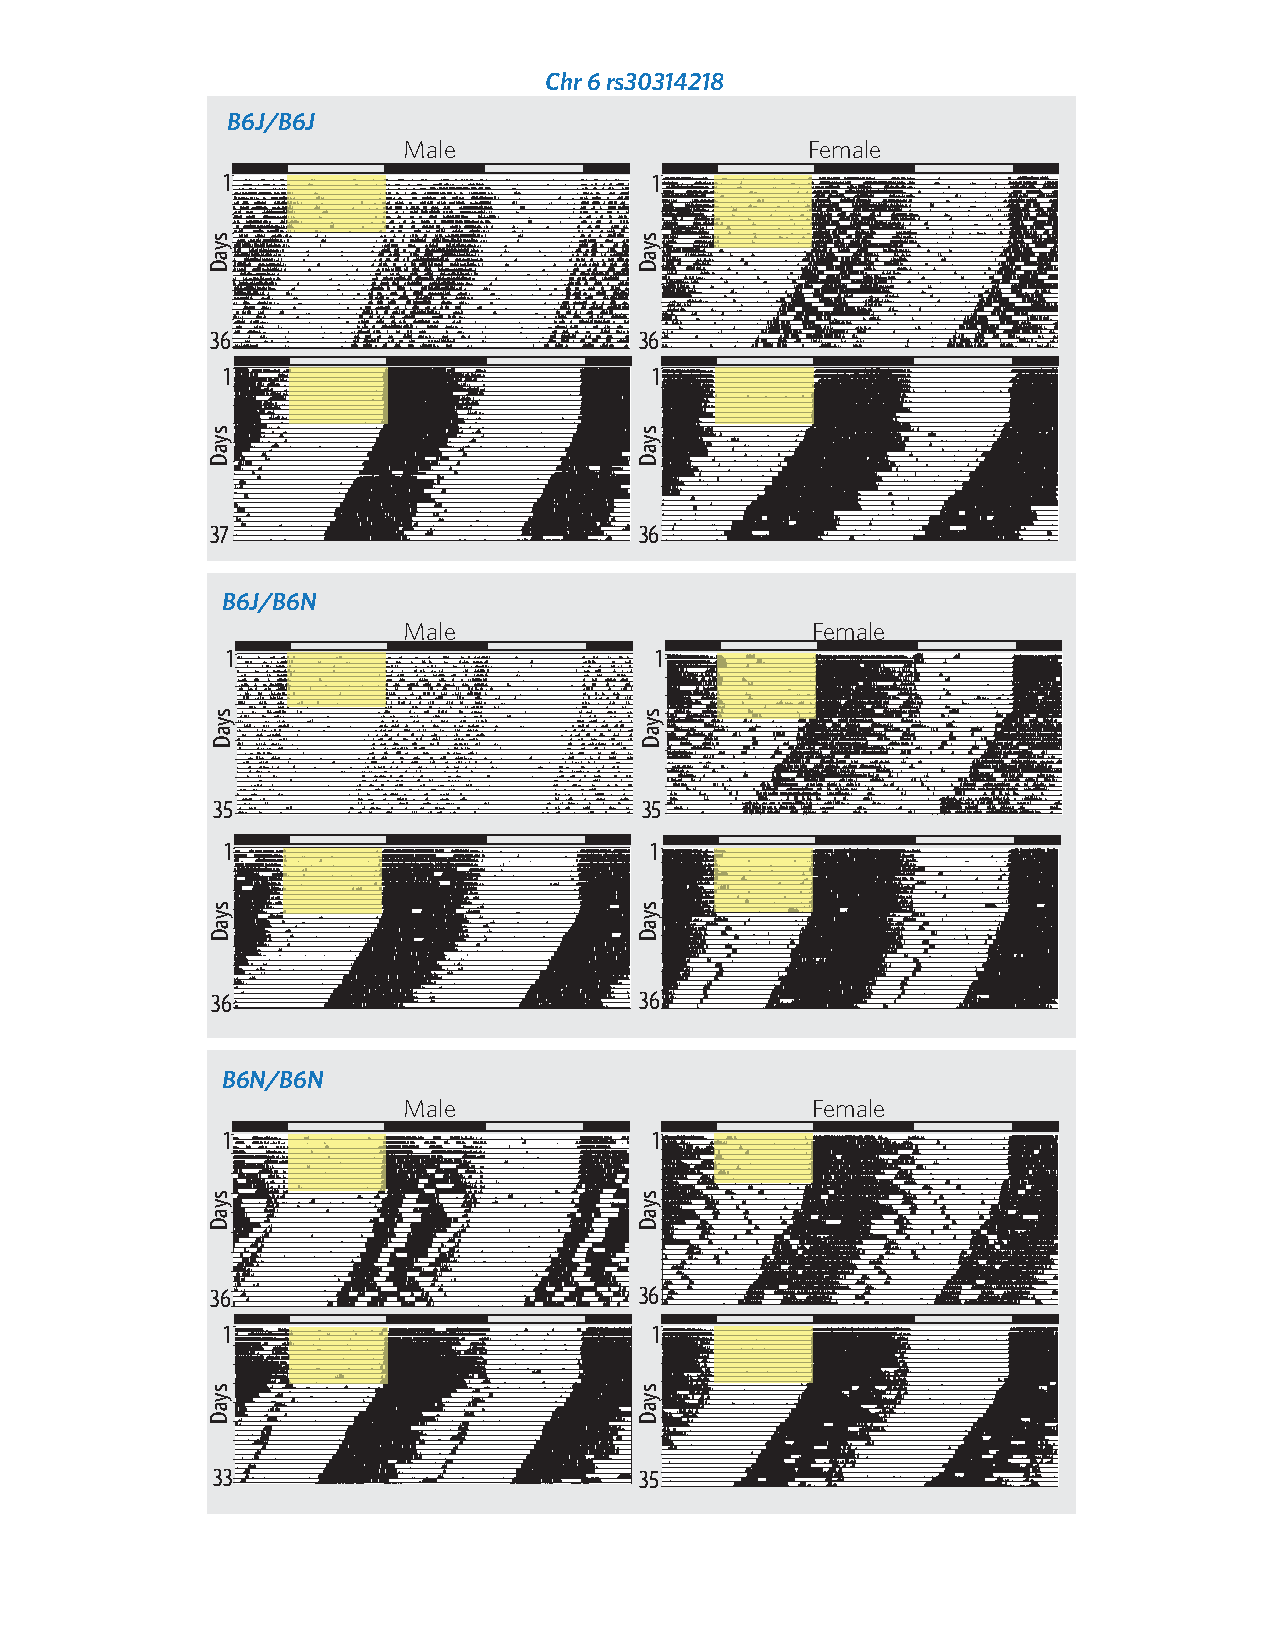
\includegraphics[width=0.6\textwidth]{images/actograms_cropped.pdf}
            \caption{
                Actograms, similar to \autoref{fig:actograms}, including female mice.
                The mice depicted here are highlighted with larger circles in \autoref{fig:kumar_phenotype_plot}.
            }
            \label{fig:actogram_supp}
        \end{figure*}

        \begin{table}
            \centering
            \caption{The characteristics of the mice plotted in \autoref{fig:actograms}}
            \begin{tabular}{p{2.5cm}lp{3cm}}
                \hline
                genotype at \newline rs30314218 & sex & activity in the DD (rev/min)\\
                % \begin{tabular}{@{}l@{}}genotype at \\ rs30314218\end{tabular}  & sex & \begin{tabular}{@{}r@{}}activity \\ in the DD (rev/min)\end{tabular} \\ 
                \hline
                6J & female & 12.79 \\ 
                6J & female & 38.20 \\ 
                6J & male & 8.07 \\ 
                6J & male & 27.99 \\ 
                Het & female & 14.03 \\ 
                Het & female & 40.13 \\ 
                Het & male & 1.87 \\ 
                Het & male & 30.68 \\ 
                6N & female & 22.22 \\ 
                6N & female & 33.85 \\ 
                6N & male & 16.75 \\ 
                6N & male & 28.71 \\ 
            \hline
        \end{tabular}
        \label{tab:acto_mice}
    \end{table}

    \newpage

    % \includepdf[pages={-}]{kumar_alignment_supplement}
    \begin{figure}
        \includegraphics[width=0.8\linewidth]{images/kumar_alignment_supplement.pdf}
        \caption{Page one of \textit{Mkrn1} alignment.  Note that the amino acid at position 346 is conserved across all species.  See next page for species labels.}
        \label{fig:mkrn1_alignment}
    \end{figure}

    \newpage
    \begin{figure}
        \includegraphics[width=0.8\linewidth]{images/kumar_alignment_supplement_p2.pdf}
        \caption{Page two of \textit{Mkrn1} alignment.}
        \label{fig:mkrn1_alignment2}
    \end{figure}



    \newpage
    \subsection{Additional Information on Bailey Reanalysis}
        \begin{figure*}
            \includegraphics[width=\textwidth]{images/bailey_replication_scanones.pdf}
            \caption{Replication of genome scans from original Bailey analysis. LOD curves are visually identical to originally-published LOD curves, but thresholds, estimated based on the described methods, are meaningfully higher.}
            \label{fig:Bailey_replicate}
        \end{figure*}

        \newpage
        \begin{figure*}
            \includegraphics[height=0.9\textheight]{images/bailey_scans_rint.pdf}
            \caption{DGLM-based reanalysis of all traits measured in Bailey et al., all transformed by the rank-based inverse normal transform.}
            \label{fig:Bailey_rint_scans}
        \end{figure*}

        \newpage
        \begin{figure*}
            \includegraphics[height=0.9\textheight]{images/bailey_scans_bc.pdf}
            \caption{DGLM-based reanalysis of all traits measured in Bailey et al., all transformed by the Box-Cox transform.  Box-Cox exponents were 1, 1, 0, 0.75, 0, 0.25, respectively.}
            \label{fig:Bailey_bc_scans}
        \end{figure*}

        \newpage
        \begin{figure*}
            \centering
            \begin{subfigure}{0.9\textwidth}
                \includegraphics[width=\textwidth]{images/TOTREAR_no_transform.pdf}
                \caption{``Rearing'' trait analyzed with no transformation.}
                \label{fig:Bailey_totrear_id}
            \end{subfigure}\\
            \begin{subfigure}{0.9\textwidth}
                \includegraphics[width=\textwidth]{images/TOTREAR_sqrt.pdf}
                \caption{``Rearing'' trait analyzed with square root transformation.}
                \label{fig:Bailey_totrear_squareroot}
            \end{subfigure}\\
            \begin{subfigure}{0.9\textwidth}
                \includegraphics[width=\textwidth]{images/TOTREAR_log.pdf}
                \caption{``Rearing'' trait analyzed with log transformation.}
                \label{fig:Bailey_totrear_log}
            \end{subfigure}\\
            \begin{subfigure}{0.9\textwidth}
                \includegraphics[width=\textwidth]{images/TOTREAR_poisson.pdf}
                \caption{``Rearing'' trait analyzed with Poisson generalized linear model.}
                \label{fig:Bailey_totrear_poisson}
            \end{subfigure}
            \caption{vQTL for TOTREAR phenotype on chromosome 2 is consistent across various transforms.}
            \label{fig:Bailey_totrear_transforms}           
        \end{figure*}
